\documentclass[hideothersubsections, usenames,dvipsnames,11pt]{beamer}
%%%%%%%%%%%%%%%%%%%%%%%%%%%%%%%%%%%%%%%%%%%%%%%%%%%%%%%%%%%%%%%%%%%%%%%%%%%%%%%%%%%%%%%%%%%%%%%%%%%%%%%%%%%%%%%%%%%%%%%%%%%%%%%%%%%%%%%%%%%%%%%%%%%%%%%%%%%%%%%%%%%%%%%%%%%%%%%%%%%%%%%%%%%%%%%%%%%%%%%%%%%%%%%%%%%%%%%%%%%%%%%%%%%%%%%%%%%%%%%%%%%%%%%%%%%%
\usepackage{algorithm}
\usepackage{algorithmic}
\usepackage{amsmath}
\usepackage{amssymb}
\usepackage{curves}
\usepackage{epic}
\usepackage{epsfig}
\usepackage{fix-cm}
\usepackage{graphicx}
\usepackage{hyperref}
\usepackage{mathpazo}
\usepackage{multimedia}
\usepackage{multicol}
\usepackage{natbib}
\usepackage{setspace}



\setcounter{MaxMatrixCols}{10}
%TCIDATA{OutputFilter=LATEX.DLL}
%TCIDATA{Version=5.00.0.2606}
%TCIDATA{Codepage=932}
%TCIDATA{<META NAME="SaveForMode" CONTENT="1">}
%TCIDATA{BibliographyScheme=Manual}
%TCIDATA{Created=Friday, November 03, 2006 10:56:24}
%TCIDATA{LastRevised=Thursday, February 19, 2015 11:02:18}
%TCIDATA{<META NAME="GraphicsSave" CONTENT="32">}
%TCIDATA{<META NAME="DocumentShell" CONTENT="Other Documents\SW\Slides - Beamer">}
%TCIDATA{Language=American English}
%TCIDATA{CSTFile=beamer.cst}

\newenvironment{stepenumerate}{\begin{enumerate}[<+->]}{\end{enumerate}}
\newenvironment{stepitemize}{\begin{itemize}[<+->]}{\end{itemize} }
\newenvironment{stepenumeratewithalert}{\begin{enumerate}[<+-| alert@+>]}{\end{enumerate}}
\newenvironment{stepitemizewithalert}{\begin{itemize}[<+-| alert@+>]}{\end{itemize} }
\newenvironment{itemize_2pt}{\itemize\addtolength{\itemsep}{2pt}}{\enditemize}
\newenvironment{enumerate_2pt}{\enumerate\addtolength{\itemsep}{2pt}}{\endenumerate}


% Color scheme
\definecolor{cerulean}{rgb}{0.16, 0.32, 0.75}
\definecolor{bdf}{rgb}{0.19, 0.55, 0.91}
\definecolor{offwhite}{RGB}{255,253,243}
\definecolor{red}{RGB}{213,94,0}
%#09BADB #DB1A71

\usetheme[right]{Berkeley}
\setbeamercolor{background canvas}{bg=offwhite}
\setbeamercolor{palette primary}{bg=cerulean,fg=white}
\setbeamercolor{palette secondary}{bg=bdf,fg=white}
\setbeamercolor{frametitle}{fg=offwhite}
%\setbeamercolor{sidebar}{bg=cerulean}
%\newenvironment{transitionframe}{\setbeamercolor{background canvas}{bg=bdf}\begin{frame}}{\end{frame}}
%\setbeamercolor{title}{fg=black}
%\setbeamercolor{itemize item}{fg=blue}
%\setbeamercolor{itemize subitem}{fg=blue}
%\setbeamercolor{enumerate item}{fg=blue}
%\setbeamercolor{enumerate subitem}{fg=blue}
%\setbeamercolor{title}{bg=red!25!blue,fg=white}
%\setbeamercolor{fo} {bg=red!25!blue,fg=white}
%\setbeamercolor{sidebar}{bg=red!25!blue,fg=white}
%\setbeamercolor{author in sidebar}{fg=black!20!white}
%\setbeamercolor{title in sidebar}{fg=white}
%\setbeamercolor{normal text}{bg=white}
%\setbeamercolor{frametitle}{fg=white}
%\setbeamercolor{section in sidebar}{bg=black,fg=white}
%\setbeamercolor{subsection in sidebar}{bg=black,fg=white}
%\setbeamercolor{block title}{bg=red!25!blue,fg=white}
%\setbeamercolor{block body}{bg=blue!20!white,fg=black}
%\setbeamerfont{subsection in sidebar}{size=\tiny}
%\setbeamerfont{title in sidebar}{size=\scriptsize}
%\setbeamerfont{author in sidebar}{size=\tiny}
%\setbeamercovered{transparent}
\setbeamercolor{section in sidebar}{bg=bdf,fg=offwhite}
\setbeamercolor{subsection in sidebar}{bg=bdf,fg=offwhite}
\setbeamercolor{button}{bg=bdf,fg=offwhite}


% Create subsection transitions without subsection numbering
\def\subsectionname{\translate{Subsection}}
\def\insertsubsectionnumber{\arabic{subsection}}
\setbeamertemplate{subsection page}
{
  %\begin{centering}
    %{\usebeamerfont{subsection name}\usebeamercolor[fg]{subsection name}\subsectionname~\insertsubsectionnumber}
    %\vskip1em\par
    \begin{beamercolorbox}[sep=14pt,center]{part title}
    	%\setbeamercolor{box1}{fg=yellow, bg=yellow}
    	\setbeamerfont{subsection title}{size=\fontsize{14}{20}\selectfont}
    	\usebeamerfont{subsection title}\insertsubsection\par
    \end{beamercolorbox}
  %\end{centering}
}
\def\subsectionpage{\usebeamertemplate*{subsection page}}
\AtBeginSubsection
{\frame{\subsectionpage}}


% Font
\usefonttheme{serif}
\setbeamercovered{invisible}
\setbeamerfont{section in sidebar}{size=\fontsize{5.3}{5}\selectfont}
\setbeamerfont{subsection in sidebar}{size=\fontsize{4.4}{5.5}\selectfont}
%\setbeamerfont{subsubsection in sidebar}{size=\fontsize{4}{7}\selectfont}
\setbeamerfont{title in sidebar}{}
\setbeamerfont{author in sidebar}{}
\setbeamerfont{itemize/enumerate body}{size={\fontsize{9.5}{9.5}}}
\setbeamerfont{itemize/enumerate subbody}{size={\fontsize{8}{8}}}
%\setbeamerfont{itemize/enumerate subbody}{family=\sffamily}
\setbeamerfont{button}{size={\fontsize{8}{8}}}
\linespread{1.25}


% Page number and navigation
\setbeamerfont{page number in head/foot}{size=\small}
%\setbeamertemplate{footline}[frame number]
\setbeamertemplate{navigation symbols}{}

\addtobeamertemplate{footline}
{%
   \usebeamercolor[fg]{author in sidebar}
   \vskip-1cm\hskip8pt
   \insertframenumber\,/\,\inserttotalframenumber\kern1em\vskip4pt%
}


% Mini frames
%\useoutertheme[subsection=true]{miniframes} 


% Bibliography
%\renewcommand\bibliographytypesize{\small}
\renewcommand*{\bibfont}{\scriptsize}


\title[]{Skills, Practices, and Aspirations \\ of Small-scale Entrepreneurs \\ in Low-income Settings}
\author[]{Julius R{\"u}schenp{\"o}hler\inst{}}
\institute[]{\inst{} UC Berkeley, CEGA}
\date{March 04, 2021}


\begin{document}


\section{\textbf{PART I: Lecture} \\ \quad \emph{Business Practices and Training}}


\setbeamertemplate{sidebar right}{}

\begin{frame}
\titlepage
\end{frame}


\setbeamertemplate{sidebar right}[sidebar theme]

\begin{frame}{Lecture Overview}
\tableofcontents[currentsection,hideothersubsections]
\end{frame}


\subsection{Business Practices Around the World}

\begin{frame}
\frametitle{Heterogeneity in Business Practices}
	\begin{itemize_2pt}
	\item Bloom and van Reenen (2010, 2019): Business practices, motivation \citep{Bloom2010, Bloom2019}
	\vspace{0.1in}
	\end{itemize_2pt}
\end{frame}

\begin{frame}
\frametitle{Heterogeneity in Business Practices}
	\begin{itemize_2pt}
	\item Bloom and van Reenen (2010): Heterogeneity across mid-sized and large firms \citep{Bloom2010}
	\end{itemize_2pt}
\end{frame}


%---------------------

\begin{frame}
\frametitle{Business Practices in Small Firms}

	\citet{McKenzie2017} develop measurement instrument of \textcolor{bdf}{26 business practices} 
	\begin{itemize_2pt}
		\item Administered in \textcolor{bdf}{7 countries} in Asia, Africa, and South America
		
\vspace{0.5em}		
		
		\item 4 major domains of business practices
		\begin{enumerate_2pt}
			\item Book-keeping and accounting
			\item Financial planning
			\item Inventory management and stock control
			\item Marketing
		\end{enumerate_2pt}
	\item[] $\rightarrow$ \textcolor{bdf}{Vast heterogeneity} in business practices \citep[comp.][]{Bloom2010}
	\item[] $\rightarrow$ \textcolor{bdf}{Strong persistent component} one year out ($r=0.59$)
	\end{itemize_2pt}
\end{frame}


\begin{frame}
\frametitle{Business Practices in Small Firms}
	\citet{McKenzie2017} identify set of XX practices most closely associated with business performance
	\begin{itemize_2pt}
		\item Example practices:
		\begin{enumerate_2pt}
			\item e.g., 
			\item e.g., 
			\item e.g., 
			\item e.g.,  
		\end{enumerate_2pt}
	\end{itemize_2pt}
\end{frame}


\begin{frame}
\frametitle{Business Practices in Small Firms}

\begin{figure}[htbp]
	\centering
	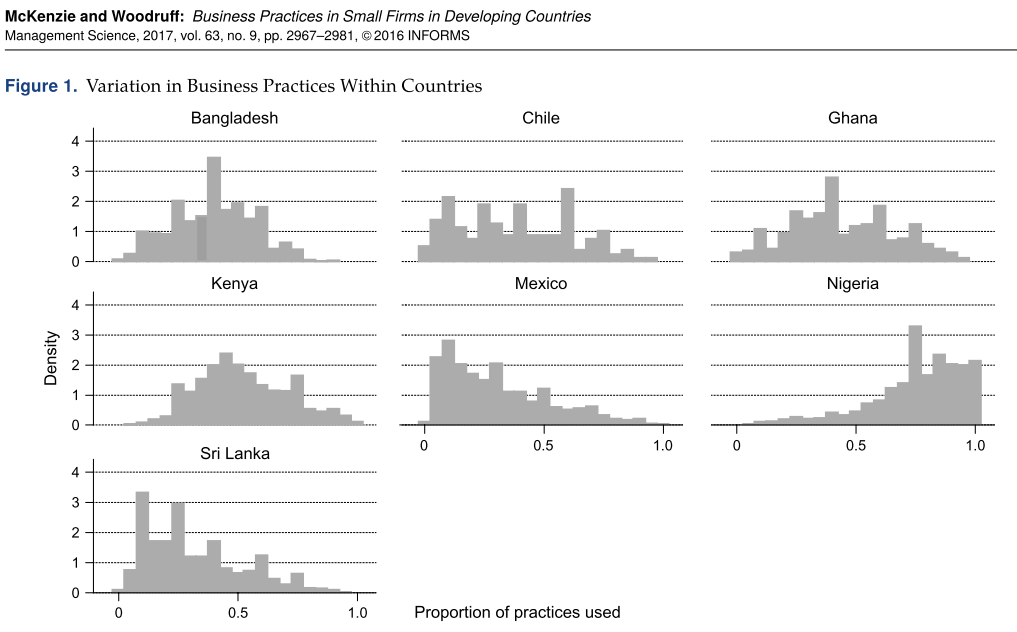
\includegraphics[width=23em]{pics/McKenzie2017_het.png}
	\label{McKenzie(2017): Heterogeneity}
\end{figure}

\begin{itemize_2pt}
	\item Hetereogeneity in business practices of MSEs across countries \citep{McKenzie2017}
\end{itemize_2pt}
\end{frame}


\begin{frame}
\frametitle{Business Practices in the Production Decision}

Standard Production Decision
	\begin{itemize_2pt}
		\item Owner maximizes output $Y = f(\textcolor{red}{A}, \textcolor{bdf}{L, M, K})$ at given wealth $\textcolor{red}{W}$:	
		
		\item[] $\boxed{ \begin{aligned} \max _{\textcolor{bdf}{K, M, L}} &\{\textcolor{red}{p} \text{ } f(\textcolor{red}{A}, \textcolor{bdf}{L, M, K})-\textcolor{red}{w} \textcolor{bdf}{L}-\textcolor{red}{s} \textcolor{bdf}{M}-\textcolor{red}{r} \textcolor{bdf}{K}\} \end{aligned} }$
		\item[] $\boxed{ \begin{aligned} \text{s.t.} &\ \textcolor{red}{w} \textcolor{bdf}{L}+\textcolor{red}{s} \textcolor{bdf}{M}+\textcolor{red}{r} \textcolor{bdf}{K} \leq \textcolor{red}{\lambda} \textcolor{red}{W} \end{aligned} }$
		
		\vspace{0.5em}		
		
		\begin{itemize_2pt}
			\item[] .. where $\textcolor{bdf}{L}$ is labor, $\textcolor{bdf}{M}$ is materials, and $\textcolor{bdf}{K}$ is capital.
			\item[] .. where $\textcolor{red}{p}$ is the output price, $\textcolor{red}{w}$ the cost of labor, $\textcolor{red}{s}$ the cost of raw materials, and $\textcolor{red}{r}$ cost of capital
			\item[] .. where $\textcolor{red}{A}$ represents a productivity factor and \textcolor{red}{$\lambda$} parameterizes borrowing constraints
		\end{itemize_2pt}	
		
		\vspace{0.5em}	
		
		\item 2 general conceptualizations of business practices
		\begin{enumerate_2pt}
			\item As factor of production $\textcolor{bdf}{B}$ chosen by owner at market price $\textcolor{red}{p_{B}}$
			\item As technology boosting productivity factor $\textcolor{red}{A}$
			\item[] \citep[see,][]{Bloom2016, McKenzie2017}
		\end{enumerate_2pt}
		
	%\item Bloom et al. (2016) Bloom N, Sadun R, Van Reenen J (2016) Management as a technol- ogy? NBERWorking Paper 22327, National Bureau of Economic Research, Cambridge, MA.
	%\item McKenzie2017 3.1.
	\end{itemize_2pt}

\end{frame}

\begin{frame}
\frametitle{Business Practices in the Production Decision}

Further specific channels of impact
\begin{enumerate_2pt}
	\item Better negotiation practices may affect raw material prices $\textcolor{red}{s}$
	\item Record-keeping and financial planning practices may affect borrowing constraints $\textcolor{red}{\lambda}$ through banks' willingness to lend
	\item Marketing practices may affect output price $\textcolor{red}{p}$ by changing demand

	\item[] $\rightarrow$ Plausible association between business practices and revenues, profits, and business growth
	\item[] $\rightarrow$ Prices ($\textcolor{red}{p}$, $\textcolor{red}{s}$, and $\textcolor{red}{p_{B}}$) and inputs ($\textcolor{bdf}{K}$, $\textcolor{bdf}{L}$, and $\textcolor{bdf}{M}$) likely endogenous to business practices $\textcolor{bdf}{B}$
\end{enumerate_2pt}

\end{frame}



\begin{frame}
\frametitle{Business Practices and Performance}
	\begin{itemize_2pt}
	\item Bloom and van Reenen (2019): Correlation with productivity across mid-sized and large firms \citep{Bloom2019}
	\item McKenzie2017: \textcolor{bdf}{Robust association with performance and firm survival} across industries and contexts in small firms
	\end{itemize_2pt}
	
\vspace{0.1in}	
	
	Open questions
	\begin{itemize_2pt}
		\item Does adoption of "best practices" \emph{cause} performance to increase?
		\item How can adoption of practices best be encouraged?
	\end{itemize_2pt}	
	
\end{frame}


\subsection{Classical MSME Training}

\begin{frame}
\frametitle{History and Prevalence}
	\begin{itemize_2pt}
		\item At least \textcolor{bdf}{USD 1 billion per year} (to 4-5 million entrepreneurs; \citet{McKenzie2020})
		\item Classical training programs \emph{precede} evidence that business practices vary and are predictive for productivity
		
		\vspace{0.5em}		
		
		\item Examples:
		\begin{itemize_2pt}
			\item Start and Improve Your Business (ILO)
			\item Business Edge (IFC)
			\item EMPRETEC Entrepreneurship Training Workshop (UNCTAD)
		\end{itemize_2pt} 
	\end{itemize_2pt}
\end{frame}

%----------------------

\begin{frame}
\frametitle{Typical Training Program}
	Content
	\begin{itemize_2pt}
	%\textcolor{}{}
	\item \textcolor{red}{Training is delivered by 600 local certified trainers and by a pool of approximately 60 international master trainers. All trainers are also entrepreneurs.
	\item Empretec Training Workshops offer different levels of instruction that include:
	\item 6-day courses (48 hours); 32-hour (usually spread over 4 days) for micro-entrepreneurs with low levels of literacy; Interactive coaching based on real business challenges of participants.}
	\end{itemize_2pt}
\end{frame}

\begin{frame}
\frametitle{Typical Training Program}
	Delivery 
	\begin{itemize_2pt}
	\item %\textcolor{}{}
	\vspace{0.1in}
	\end{itemize_2pt}
\end{frame}

%---------------------

\begin{frame}
\frametitle{Impact on Performance}
	\begin{itemize_2pt}
	\item First wave (Karlan and Valdivia, 2011, Bruhn and Zia, 2013; Giné and Mansuri, 2014; Field, et al., 2010; Bulte et al., 2017; Anderson, Chandy, and Zia, 2018)
					 \citep{Karlan2011} \citep{Field2010} \citet{Gine2014} \citep{Bruhn2013} \citep{Bulte2017} \citep{Anderson2018}
	\vspace{0.1in}
	\end{itemize_2pt}
\end{frame}

\begin{frame}
\frametitle{Impact on Performance}
	\begin{itemize_2pt}
	\item Econometric and implementation issues \citep{McKenzie2014}
	\vspace{0.1in}
	\end{itemize_2pt}
\end{frame}

\begin{frame}[label=McK2020_profits]
\frametitle{Impact on Performance}
	
	Including more recent evaluations \citep[see,][]{McKenzie2020}
	
\vspace{-0.5em}	
	
	\begin{figure}[htbp]
		\centering
		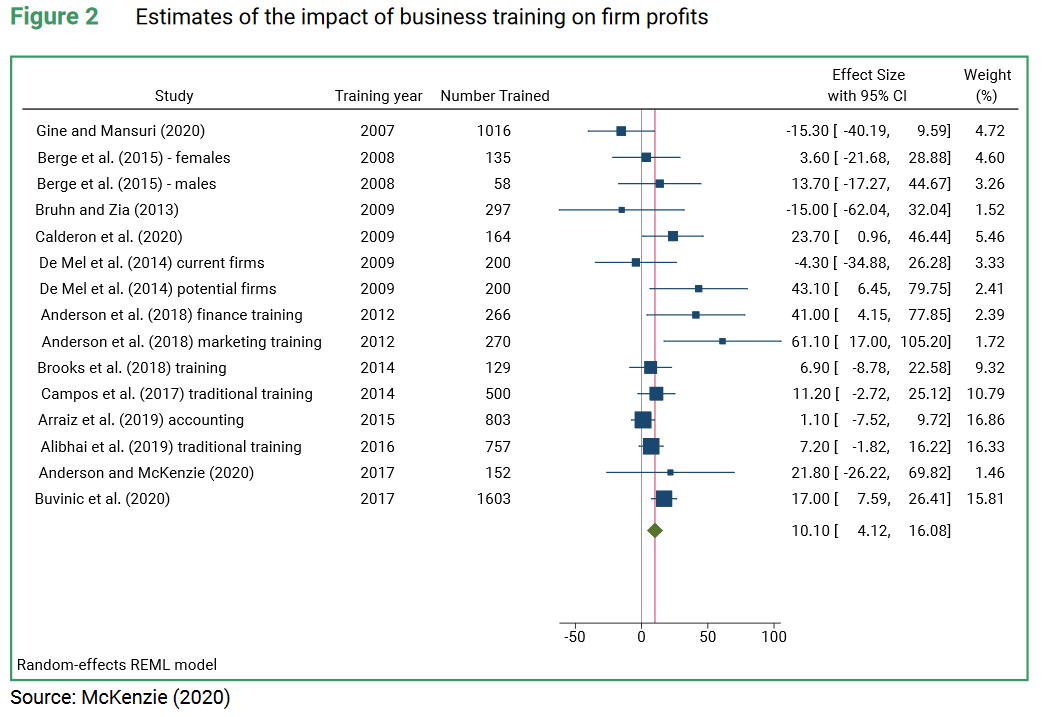
\includegraphics[width=21.5em]{pics/McK2020_profits.png}
		\label{McKenzie(2020): Profits}
	\end{figure}	
	
	\vspace{-1em}	
	
	\begin{itemize_2pt}
		\item Small positive impact on practice adoption, profits, and \hyperlink{McK2020_sales}{\beamergotobutton{sales}}
	\end{itemize_2pt}
	
	%Right side pics
	%\begin{tikzpicture}[remember picture, overlay]
		%\node[shift={(-6.5em,1em)}]() at (current page.south east){%
		%\hyperlink{appendix_sales}{\beamergotobutton{Sales}}};        
	%\end{tikzpicture}
	
\end{frame}

\begin{frame}
\frametitle{Targeted Training}
	Refinements of the classical model
	
	\vspace{0.5em}
	
	\begin{itemize_2pt}
		\item Targeting \textcolor{bdf}{specific subgroups} of the population
		\begin{itemize_2pt}
			\item Alleviating \textcolor{bdf}{particularly severe constraints}
			\item[] $\rightarrow$ Marginalized or disadvantaged groups (e.g., women, youth)
			\item  Maximizing \textcolor{bdf}{treatment impact} or cost-effectiveness 
			\item[] $\rightarrow$ Promising entrepreneurs (e.g., high-growth firms)
			
			\vspace{0.5em}			
			
			\item Plus: \textcolor{bdf}{Maximizing statistical power} through homogeneity
		\end{itemize_2pt}
		
	\vspace{1.0em}		
		
		\item Training of skills in \textcolor{bdf}{particular domains}
		\begin{itemize_2pt}
			\item Alleviating \textcolor{bdf}{specific constraints}
			\item Investigating mechanisms of treatment impact
		\end{itemize_2pt}
	\end{itemize_2pt}
\end{frame}

\begin{frame}
\frametitle{Targeted Training}
	Female entrepreneurs
	\begin{itemize_2pt}
		\item \textcolor{bdf}{Most common type of targeted training} (potentially complementary to classical microfinance model)
		\item Example: Gender and Enterprise Together \citep[GET Ahead, ILO;][]{Bulte2016,McKenziePuerto2020}
		\item ?
	\vspace{0.1in}
	\end{itemize_2pt}
\end{frame}

\begin{frame}
\frametitle{Targeted Training}
	Young entrepreneurs
	\begin{itemize_2pt}
		\item Typically embedded as entrepreneurship programs in school and university
		\item Example: University final year course in Tunisia \citep{Alaref2020}
		\begin{itemize_2pt}
			\item
			\item
		\end{itemize_2pt}
	\end{itemize_2pt}
\end{frame}

\begin{frame}
\frametitle{Targeted Training}
	High-growth businesses ("gazelles")
	\begin{itemize_2pt}
	\item Marcel Fafchamps and Simon Quinn, \citep{McKenzie2017a}
	\item Small literature on business accelerators and incubators \citep[see, e.g.,][]{Cusolito2020, Gonzalez-Uribe2017, Gonzalez-Uribe2020}
	\vspace{0.1in}
	\end{itemize_2pt}
\end{frame}

%---------------------

\begin{frame}
\frametitle{Training Specific Domains}

	\citet{Anderson2018} assign 852 South African MSEs to distinct types of training:
	\begin{enumerate_2pt}
		\item Marketing/sales skills
		\item[]
		\item[]
		\item Finance/accounting skills
		\item[]
		\item[]
	\end{enumerate_2pt}

\end{frame}


\begin{frame}
\frametitle{Training Specific Domains}

	\citet{Anderson2018} assign 852 South African businesses to two distinct trainings:
	\begin{enumerate_2pt}
	
		\item Marketing/sales skills
		\begin{itemize_2pt}
			\item 61\% increase in profits
			\item "Growth focus" on higher sales, stock investments, and hiring
			\item[] $\rightarrow$ Benefits new businesses ($=$ less market exposure)
		\end{itemize_2pt}		
		
		\item Finance/accounting skills
		
		\pause		
		
		\begin{itemize_2pt}
			\item 41\% increase in profits
			\item "Efficiency focus" on lower costs
			\item[] $\rightarrow$ Benefits established businesses
		\end{itemize_2pt}
		
		\item[] $\rightarrow$ Different "pathways to profits"
	
	\end{enumerate_2pt}

\end{frame}


\subsection{Extensions of the Classical Approach}

\begin{frame}
\frametitle{On-site Consulting}

Typical Consulting Intervention
\begin{itemize_2pt}
	\item Three-step procedure
	\begin{enumerate_2pt}
		\item Diagnostic of practices
		\item Identification of areas of improvement
		\item Problem solving within interactive relationship
	\end{enumerate_2pt}
	
	\pause
	
	\item \textcolor{bdf}{Sustained and intensive}
	\begin{itemize_2pt}
		\item Total of 88 to 200 hours and more \citep{Anderson2020, Bruhn2018, Karlan2015, Bruhn2019}
		\item[] $\rightarrow$ Typically several months
		\item[] $\rightarrow$ Meetings monthly to twice weekly, 2-4 hours
		\item Total cost between \textcolor{red}{USD 4,000 and 12,000 per firm} \citep{Anderson2020, Bruhn2018}
	\end{itemize_2pt}
	
	\pause
	
	\item Typically one-on-one (also group-based)
	
	\item \textcolor{bdf}{Often gov't-subsidized} (private contributions typically around 10\%)
	\begin{itemize_2pt}
		\item Empirical finding: Firms often unwilling to pay market price \citep{Maffioli2020}
		\item[] $\rightarrow$ \textcolor{bdf}{Matching-grant programs}
	\end{itemize_2pt}
	
\end{itemize_2pt}
\end{frame}


\begin{frame}
\frametitle{On-site Consulting}

SME consulting \citep{Bruhn2018}
\begin{itemize_2pt}
	\item Evaluation of a matching grants program in Mexico
	\begin{itemize_2pt}
		\item
	\end{itemize_2pt}
\end{itemize_2pt}


\end{frame}

%---------------------

\begin{frame}
\frametitle{Multimedia delivery}
	TV shows
	\begin{itemize_2pt}
	\item Examples: Ruka Juu in Tanzania \citep{Bjorvatn2020} and El Mashroua in Egypt \citep{Barsoum2018}
	\item ?
	\vspace{0.1in}
	\end{itemize_2pt}
\end{frame}

\begin{frame}
\frametitle{Multimedia delivery}
	TV shows
	\begin{itemize_2pt}
	\item Examples: Ruka Juu in Tanzania \citep{Bjorvatn2020} and El Mashroua in Egypt \citep{Barsoum2018}
	\item ?
	\vspace{0.1in}
	\end{itemize_2pt}
\end{frame}

\begin{frame}
\frametitle{Multimedia delivery}
	Text messages
	\begin{itemize_2pt}
	\item \citep{Cole2019} \citep{Acimovic2020}
	\vspace{0.1in}
	\end{itemize_2pt}
\end{frame}

% -----------------------

\begin{frame}
\frametitle{Complementary Constraints}
	\begin{itemize_2pt}
	\item McKenzie cash JDE paper
	\vspace{0.1in}
	\end{itemize_2pt}
\end{frame}

\begin{frame}
\frametitle{Complementary Constraints}
	\begin{itemize_2pt}
	\item McKenzie cash JDE paper
	\vspace{0.1in}
	\end{itemize_2pt}
\end{frame}


\subsection{Measurement of Firm Performance}

\begin{frame}
\frametitle{Imprecision of Outcome Measures}
	
	\begin{figure}[htbp]
		\centering
		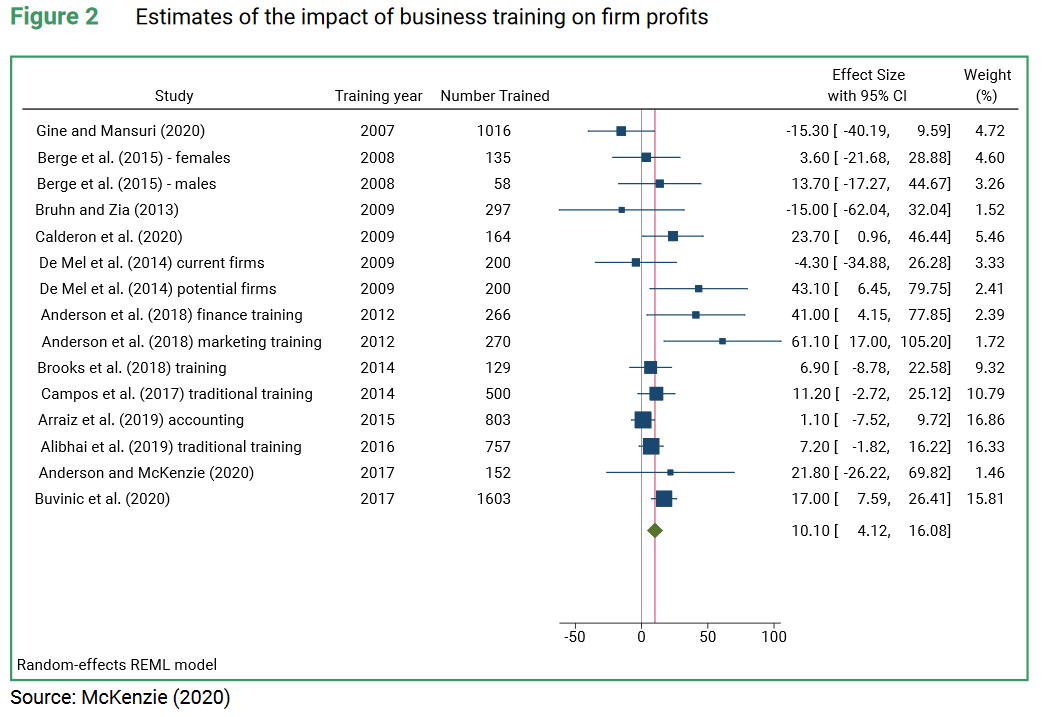
\includegraphics[width=23.5em]{pics/McK2020_profits.png}
		\label{McKenzie(2020): Profits}
	\end{figure}	
	
\vspace{-1em}	
	
	\begin{itemize_2pt}
		\item \textcolor{bdf}{Extremely wide confidence intervals} on impact estimates
	\vspace{0.1in}
	\end{itemize_2pt}
\end{frame}

\begin{frame}
\frametitle{Self-reports and aggregation}
	\begin{itemize_2pt}
	\item Self-reports of aggregate \citep{deMel2009}
	\vspace{0.1in}
	\end{itemize_2pt}
\end{frame}

\begin{frame}
\frametitle{Self-reports and aggregation}
	\begin{itemize_2pt}
	\item Disaggregating quantities in self-reports \citep{deMel2009}
	\vspace{0.1in}
	\end{itemize_2pt}
\end{frame}

\begin{frame}
\frametitle{Self-reports and aggregation}
	\begin{itemize_2pt}
	\item Direct measures \citep{deMel2009}
	\vspace{0.1in}
	\end{itemize_2pt}
\end{frame}

%---------------------

\begin{frame}
\frametitle{Sales vs. Profits}
	\begin{itemize_2pt}
	\item  \citep{deMel2009}
	\vspace{0.1in}
	\end{itemize_2pt}
\end{frame}

\begin{frame}
\frametitle{Sales vs. Profits}
	\begin{itemize_2pt}
	\item \citep{deMel2009}
	\vspace{0.1in}
	\end{itemize_2pt}
\end{frame}

% ---------------------

\begin{frame}
\frametitle{?}
\begin{itemize_2pt}
	\item 
	\vspace{0.1in}
\end{itemize_2pt}
\end{frame}

\begin{frame}
\frametitle{?}
\begin{itemize_2pt}
	\item 
	\vspace{0.1in}
\end{itemize_2pt}
\end{frame}


\subsection{Mechanisms}

\begin{frame}
\frametitle{Heterogeneity of Impact}

Heterogeneity of treatment effects poorly understood across different approaches
\begin{itemize_2pt}
	\item Potential constraints are manifold, and likely context-dependent
	
\vspace{0.5em}	
	
	\item Some more obvious constraints (already mentioned in passing):
	\begin{itemize_2pt}
		\item \textcolor{bdf}{Credit constraints} \citep[see, e.g.,][]{} McKenzie cash paper
		\item \textcolor{bdf}{Gender norms and constraints}
		\item \textcolor{bdf}{Age-related} network and knowledge/skill \textcolor{bdf}{constraints}
	\end{itemize_2pt} 
\end{itemize_2pt}
	
	\vspace{1.0em}

$\rightarrow$ More recent literature highlights \textcolor{bdf}{behavioral constraints}

\end{frame}

\begin{frame}
\frametitle{Education and literacy}

Most MSE entrepreneurs have limited education

\vspace{-1.9em}

\begin{figure}[htbp]
	\centering
	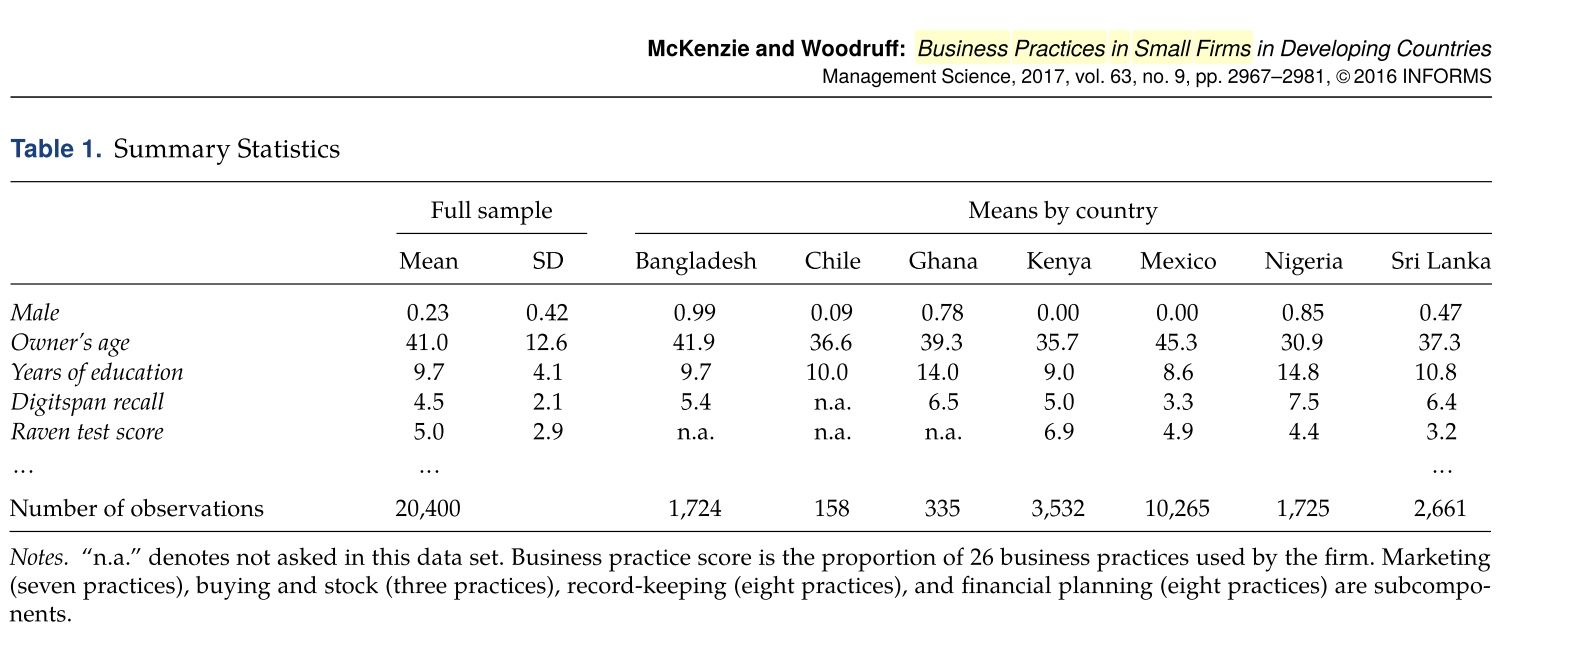
\includegraphics[width=27em]{pics/McK2017_educ.png}
	\label{McKenzie(2017): Education and cognitive functioning}
\end{figure}

\vspace{-2.5em}

\begin{itemize_2pt}
	\item Typical small-firm owner dropped out of highschool
	\item Test scores on digitspan and Raven's matrices about \% of Western university samples \textcolor{red}{\citep[comp.][]{}}
\end{itemize_2pt}
\end{frame}

\begin{frame}
\frametitle{Education and literacy}

Potential for heuristics and rules of thumb
\begin{itemize_2pt}
	\item Drexler, Fischer \& Schoar (2014) \citep{Drexler2014}
	\vspace{0.1in}
\end{itemize_2pt}
\end{frame}

\begin{frame}
\frametitle{Dynamic complementarities in skill acquisition}

Complementarities in skills
\begin{itemize_2pt}
	\item
\end{itemize_2pt}

\vspace{1.0em}

Learning styles
\begin{itemize_2pt}
	\item
\end{itemize_2pt}

\end{frame}

\begin{frame}
\frametitle{Family Commitments}
\begin{itemize_2pt}
	\item Interesting; \textcolor{red}{no beh const}
	\vspace{0.1in}
\end{itemize_2pt}
\end{frame}

\begin{frame}
\frametitle{Segregated Markets}
\begin{itemize_2pt}
	\item Missing economies of scale
	\item \textcolor{red}{Interesting; not behavioral constraint}
	\vspace{0.1in}
\end{itemize_2pt}
\end{frame}

%\begin{frame}
%\frametitle{Identity Concerns}
%\begin{itemize_2pt}
%	\item 
%	\vspace{0.1in}
%\end{itemize_2pt}
%\end{frame}

\begin{frame}
\frametitle{Aspirations}
\begin{itemize_2pt}
	\item 
	\vspace{0.1in}
\end{itemize_2pt}
\end{frame}

\begin{frame}
\frametitle{Local Relevance of Business Practices}
\begin{itemize_2pt}
	\item 
	\vspace{0.1in}
\end{itemize_2pt}
\end{frame}


\subsection{Alternative Approaches}

\begin{frame}
\frametitle{Rules of Thumb}
	\begin{itemize_2pt}
	\item Drexler, Fischer \& Schoar (2014) \citep{Drexler2014}
	\vspace{0.1in}
	\end{itemize_2pt}
\end{frame}

\begin{frame}
\frametitle{Rules of Thumb}
	\begin{itemize_2pt}
	\item \citep{Arraiz2019} \citep{Cole2019}
	\vspace{0.1in}
	\end{itemize_2pt}
\end{frame}

%

\begin{frame}
\frametitle{Entrepreneurial mindset}
	\begin{itemize_2pt}
	\item \citep{Campos2017}
	\vspace{0.1in}
	\end{itemize_2pt}
\end{frame}

\begin{frame}
\frametitle{Entrepreneurial mindset}
	\begin{itemize_2pt}
	\item \citep{Alibhai2019} \citep{Ubfal2019}
	\vspace{0.1in}
	\end{itemize_2pt}
\end{frame}

%---------------------

\begin{frame}
\frametitle{Local Knowledge}
	\begin{itemize_2pt}
	\item Cai and Szeidl (2019), Brooks et al. (2018), Lafortune et al. (2020), Seither (2020), Abebe et al. (2020)?
	\vspace{0.1in}
	\end{itemize_2pt}
\end{frame}

\begin{frame}
\frametitle{Local Knowledge}
	\begin{itemize_2pt}
	\item Cai and Szeidl (2019), Brooks et al. (2018), Lafortune et al. (2020), Seither (2020), Abebe et al. (2020)?
	\vspace{0.1in}
	\end{itemize_2pt}
\end{frame}

\begin{frame}
\frametitle{Local Knowledge}
	\begin{itemize_2pt}
	\item Cai and Szeidl (2019), Brooks et al. (2018), Lafortune et al. (2020), Seither (2020), Abebe et al. (2020)?
	\vspace{0.1in}
	\end{itemize_2pt}
\end{frame}

%---------------------

\begin{frame}
\frametitle{Role Models}
	\begin{itemize_2pt}
	\item  La Ferrara et al. (2012); Chong and La Ferrara (2009); Berg and Zia (2013); Riley (2018)
	\vspace{0.1in}
	\end{itemize_2pt}
\end{frame}

\begin{frame}
\frametitle{Role Models}
	\begin{itemize_2pt}
	\item  La Ferrara et al. (2012); Chong and La Ferrara (2009); Berg and Zia (2013); Riley (2018
	\vspace{0.1in}
	\end{itemize_2pt}
\end{frame}

\begin{frame}
\frametitle{Role Models}
	\begin{itemize_2pt}
	\item  La Ferrara et al. (2012); Chong and La Ferrara (2009); Berg and Zia (2013); Riley (2018)
	\vspace{0.1in}
	\end{itemize_2pt}
\end{frame}


\addtocontents{toc}{\protect\setcounter{tocdepth}{0}}

\subsection{Takeaways}

\begin{frame}
\frametitle{Takeaways}
	\begin{itemize_2pt}
    \item
   	\vspace{0.10in}
\end{itemize_2pt}
\end{frame}

\begin{frame}
\frametitle{Questions}
	\textcolor{bdf}{Any questions?}
	\begin{itemize_2pt}
	\item[] .. before we move on to our paper?
	\end{itemize_2pt}
\end{frame}


%-----------------------------------------------------------
%------------------------------------------------------------
%------------------------------------------------------------
%------------------------------------------------------------
%------------------------------------------------------------

\addtocontents{toc}{\protect\setcounter{tocdepth}{99}}

\title[]{Curating Local Knowledge}
\subtitle{Experimental Evidence from Small Retailers in Indonesia}

\author[]
{Patricio S. Dalton\inst{1}\
Julius R{\"u}schenp{\"o}hler\inst{2}
Burak Uras\inst{1}\\and
Bilal Zia\inst{3}}

\institute[]{
\inst{1} Tilburg University \\
\inst{2} UC Berkeley, CEGA\\
\inst{3} The World Bank}

\date{March 04, 2021}


\section{\textbf{PART II: Paper} \\ \quad \emph{Curating Local Knowledge}}

\setbeamertemplate{sidebar right}{}

\begin{frame}
\titlepage
\end{frame}


\setbeamertemplate{sidebar right}[sidebar theme]

\begin{frame}{Paper Overview}
\tableofcontents[currentsection,hideothersubsections]
\end{frame}


%------------------------------------------------
\subsection{Motivation}

\begin{frame}
\frametitle{Background}
	\begin{itemize_2pt}
	\item Micro and small firms (MSEs) are typically the main \textcolor{bdf}{source of employment} in the developing world
	\item In \textcolor{bdf}{Indonesia}, MSEs represent .. 
	\begin{itemize_2pt}
		\item .. 99\% of all firms
		\item .. 94.5\% of employment
	\end{itemize_2pt} 
	\item Understanding the factors fostering efficiency and growth of MSEs is an important research and policy goal
	\end{itemize_2pt}
\end{frame}

%------------------------------------------------
\begin{frame}
\frametitle{A Growing Focus on Management}
\begin{itemize_2pt}
\item \textcolor{bdf}{Classroom Training}: Field, et al. (2010); Karlan \& Valdivia (2011); Bruhn \& Zia (2013); McKenzie \& Woodruff (2014, 2017); Bulte et al. (2017); Anderson, Chandy \& Zia (2018); Lafortune et al. (2018)
\vspace{0.1in}
\item \textcolor{bdf}{Consulting}: Bloom, et al. (2013); Karlan et al (2015); Bruhn, Karlan \& Schoar (2019)
\vspace{0.1in}

\item \textcolor{bdf}{Mobilizing Peer Knowledge}:
    \begin{itemize_2pt}
    \item Brooks et al. (2018) $\rightarrow$ Local mentors (market information)
    \item Cai \& Szeidl (2018) $\rightarrow$ Business meetings
    \item Abebe et al. (2019) $\rightarrow$ Management experience matching
    \end{itemize_2pt}
    \vspace{0.1in}
\end{itemize_2pt}
\end{frame}

\subsection{Our Approach}
\begin{frame}
\frametitle{Harnessing Cross-Firm Heterogeneity}
Some stylized facts about business practices in small firms
\begin{itemize_2pt}
	\item Vast heterogeneity in business practices and performance across similar businesses \citep{deMel2009}
	\item Variation in practices accounts for more than 20\% of variation in productivity within the same firm in the US \citep{Bloom2019}
	\item[] $\rightarrow$ Research has largely overlooked this heterogeneity in program design and implementation
\end{itemize_2pt}

\vspace{0.5em}
\pause

We \textcolor{bdf}{make productive use of this heterogeneity} in our research design: 
\begin{itemize_2pt}
	\item Use cross-firm variation to identify \textcolor{bdf}{practices associated with business performance}
	\item \textcolor{bdf}{Curation} of local best practices
	\item Test different \textcolor{bdf}{modes of delivery}, and their cost-effectiveness
\end{itemize_2pt}

\end{frame}

\begin{frame}
\frametitle{Selecting Local Best Practices}
\begin{itemize_2pt}
\item Detailed \textcolor{bdf}{qualitative interviews} with local business peers:
    \begin{itemize_2pt}
    \item Understand and codify their practices (record-keeping, financial planning, stocking-up, marketing, and joint decision-making)
    \item Identify implementation norms and beliefs regarding each practice (e.g. whether they are complicated, necessary, etc.)
    \item Document locally relevant tips and rule of thumbs
    \end{itemize_2pt}
\vspace{0.1in}
\item Baseline \textcolor{bdf}{quantitative survey}
    \begin{itemize_2pt}
    \item Measure practices and outcomes
    \item Quantitative association of business practices with profits and sales
    \end{itemize_2pt}
\end{itemize_2pt}
\end{frame}


\begin{frame}
\frametitle{Disseminating Knowledge}

	Basic information intervention
	\begin{itemize_2pt}
		\item \textcolor{bdf}{Handbook}
		\begin{itemize_2pt}
			\item \textcolor{bdf}{Pure information}: Which practices, how to adopt, and why?\\
		\end{itemize_2pt}
	\end{itemize_2pt}
	
	\vspace{1.0em}

	Two complementary behavioral interventions:
	\begin{itemize_2pt}
		\item \textcolor{bdf}{Movie}
		\begin{itemize_2pt}
			\item \textcolor{bdf}{Psychological and emotional involvement}$\rightarrow$ social learning is possible through \textcolor{bdf}{observing the successful experience of similar others}.
			\item Bernard, et al. (2014); La Ferrara et al. (2012); Chong and La Ferrara (2009); Berg and Zia (2013).\\
		\end{itemize_2pt}

		\item \textcolor{bdf}{On-site Assistance}
			\begin{itemize_2pt}
				\item \textcolor{bdf}{Hands-on involvement} $\rightarrow$ social learning is possible through own \textcolor{bdf}{experience, 					with a small nudge} (Kolb, 1984).
				\item Facilitated by local lay person
			\end{itemize_2pt}


	\end{itemize_2pt}

\end{frame}


\begin{frame}
\frametitle{Research Questions}

	\textcolor{bdf}{Characterization of local best practices}
	\begin{itemize_2pt}
		\item Which practices are associated with high profits?
		\item How do successful businesses implement them?
	\end{itemize_2pt}
	\vspace{1.0em}
	
	\textcolor{bdf}{Adoption of best practices}
	\begin{itemize_2pt}
		\item Do retailers adopt these practices once peer best practices are aggregated and made common knowledge?
		\item If so, does the type of experiential involvement matter?

	\end{itemize_2pt}
    \vspace{1.0em}
    
	\textcolor{bdf}{Impact on business performance}
	\begin{itemize_2pt}
		\item Does firm profitability increase?
		\item If so, what are the channels?
	\end{itemize_2pt}

\end{frame}

\subsection{Data and Design}

\begin{frame}
\frametitle{Sample}
\begin{itemize_2pt}
\item Listing of 2042 small retail businesses from 29 sub-districts ("kelurahan") in urban Jakarta
\item Selection criteria for firm listing:
	\begin{itemize_2pt}
%	\item General willingness to grow
	\item At least 4$m^{2}$ in size
	\item At least two different product categories on offer
	\item At least 30 meters distance to next business in sample $\rightarrow$ to minimize spillovers
	\end{itemize_2pt}
\item Random sample of 1301 from the list
\item Randomization to treatment arms stratified by
	\begin{itemize_2pt}
	\item Gender
	\item Firm space (4-6$m^2$, 6-10$m^2$, 10 and above $m^2$)
	\item Composite score of business practices above or below median
	\item Sub-district
	\end{itemize_2pt}
\end{itemize_2pt}
\end{frame}


\begin{frame}
\frametitle{Experimental Design}

	Three types of information delivery:
		\begin{enumerate_2pt}
			\item \textcolor{bdf}{Handbook} with best practices and implementation tips
			\item \textcolor{bdf}{Movie} with successful peers
			\item \textcolor{bdf}{On-site assistance} with practice adoption
			\item[] $\rightarrow$ Movie, assistance exclusively based on handbook
		\end{enumerate_2pt}
	\vspace{0.1in}
	
	Five experimental groups
    	\begin{enumerate_2pt}
        	\item \textcolor{bdf}{Handbook} only (N=260)
        	\item \textcolor{bdf}{Handbook} + invitation to \textcolor{bdf}{movie} screening (N=260)
        	\item \textcolor{bdf}{Handbook} + offer of two \textcolor{bdf}{assistance} visits (N=260)
        	\item \textcolor{bdf}{Handbook} + \textcolor{bdf}{movie} + \textcolor{bdf}{assistance} (N=260)
       		\item Control (N=261)
      	\end{enumerate_2pt}
\end{frame}


\begin{frame}
\frametitle{Timeline}
\begin{enumerate_2pt}
    \item September 2015: \textcolor{bdf}{Qualitative} Interviews
    \item January 2016: \textcolor{bdf}{Firm listing} ($\rightarrow$ survey instrument)
    \item Feb-Apr 2016: \textcolor{bdf}{Baseline} survey
    \item Oct-Nov 2016: \textcolor{bdf}{Interventions}
    \item Apr-May 2017: \textcolor{bdf}{Midline} survey
    \item Apr-May 2018: \textcolor{bdf}{Endline} survey
\end{enumerate_2pt}
\end{frame}


\begin{frame}
\frametitle{Typical Business in the Sample}

\begin{figure}[htbp]
	\centering
		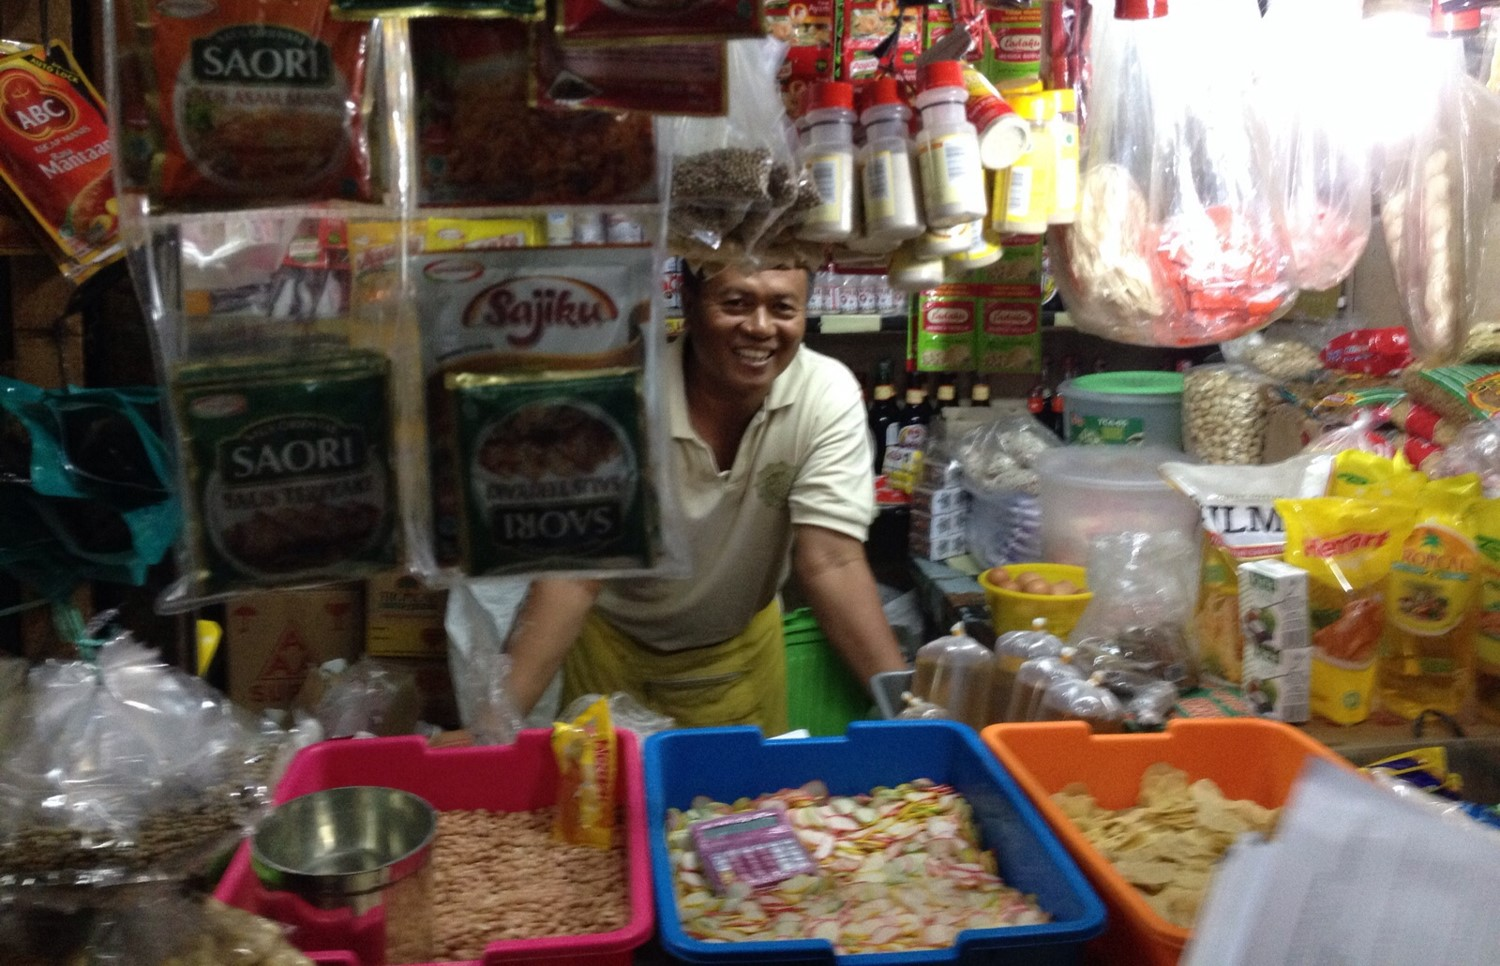
\includegraphics[width=4in]{pics/retailer1.jpg}
	%\caption{Best-practices handbook}
	\label{height}
\end{figure}
\end{frame}

\begin{frame}
\frametitle{Typical Business in the Sample}

\begin{figure}[htbp]
	\centering
		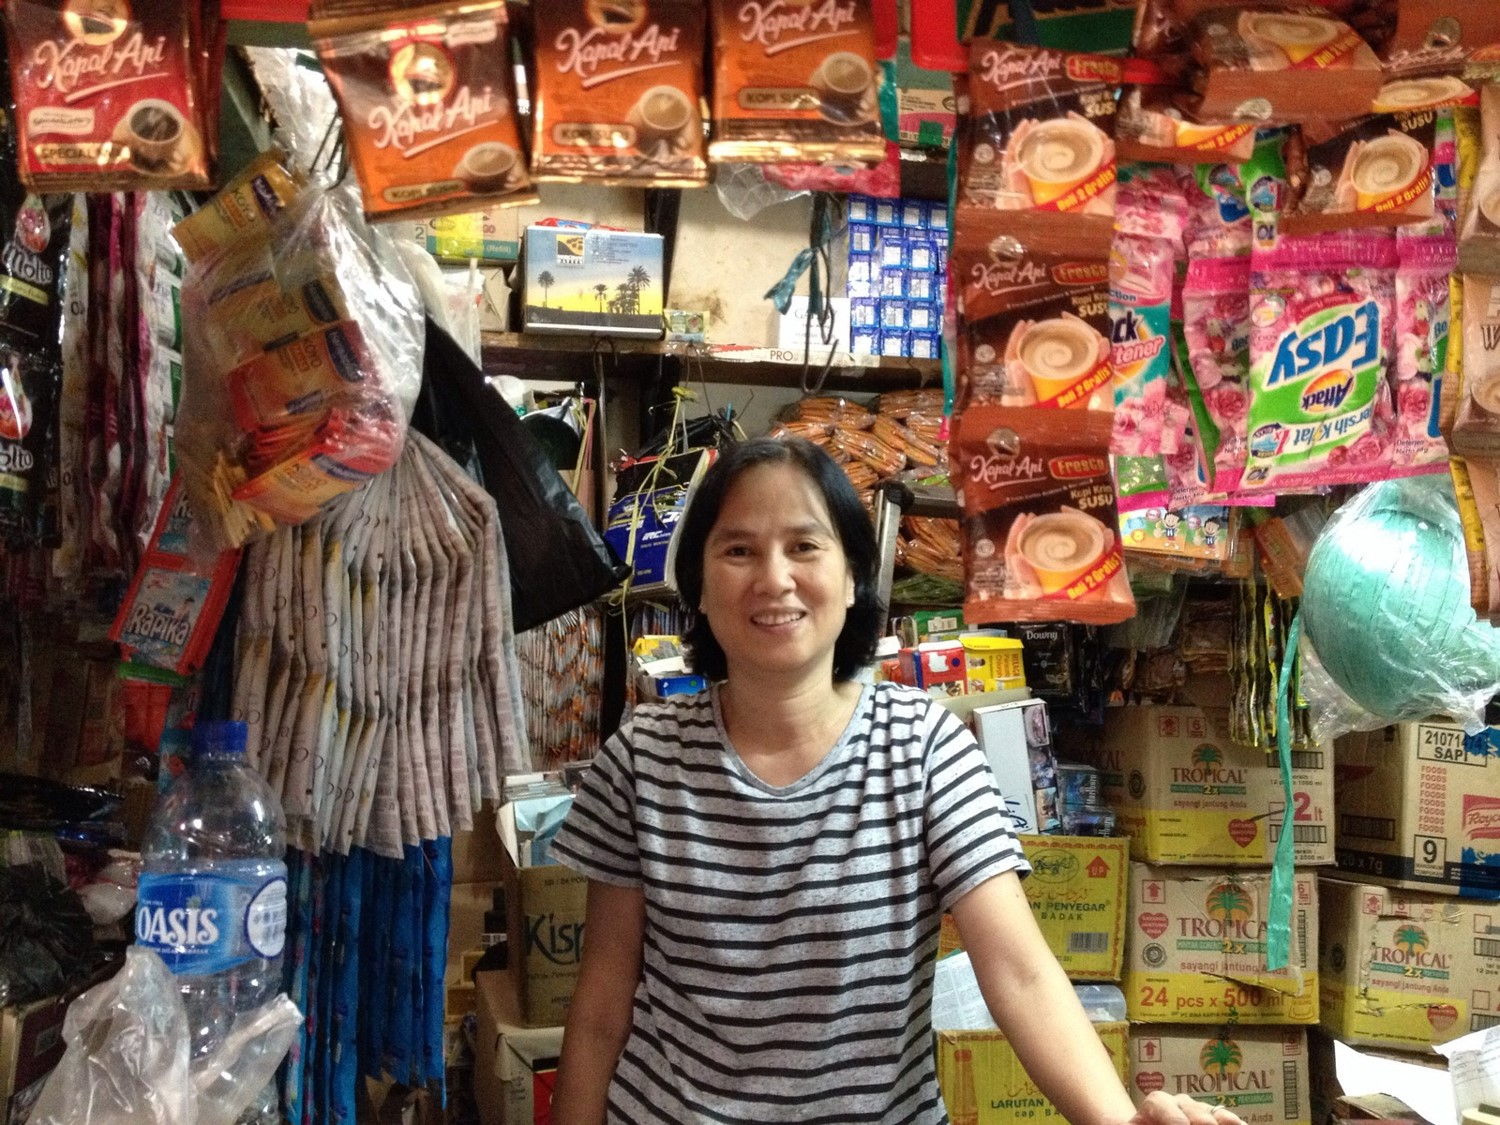
\includegraphics[width=4in]{pics/retailer2.jpg}
	%\caption{Best-practices handbook}
	\label{height}
\end{figure}
\end{frame}


\begin{frame}
\frametitle{Best-practices Handbook}

\begin{figure}[htbp]
	\centering
		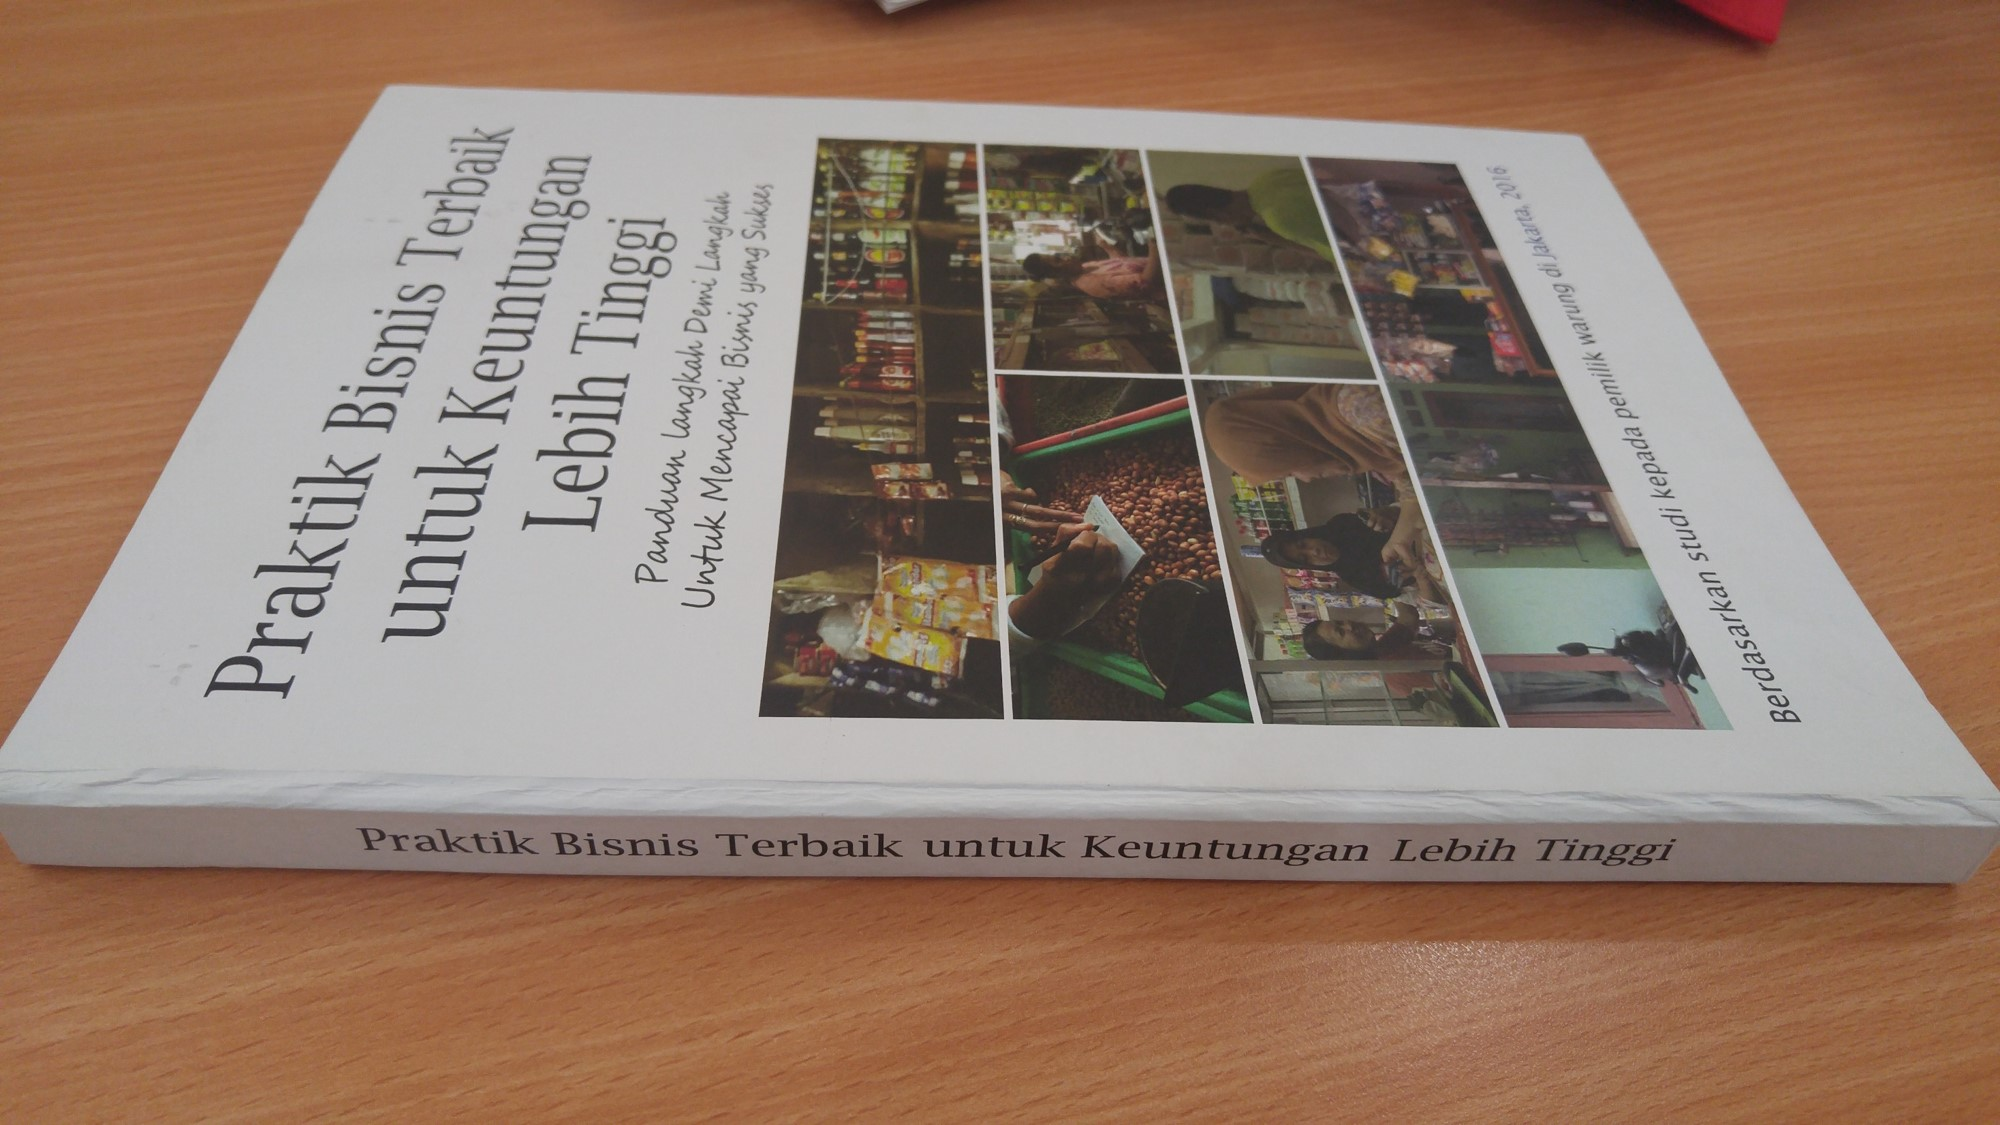
\includegraphics[width=4in]{pics/handbook.jpg}
	
	\label{height}
\end{figure}
\end{frame}


\begin{frame}
\frametitle{Handbook Content}
\begin{figure}[htbp]
	\centering
		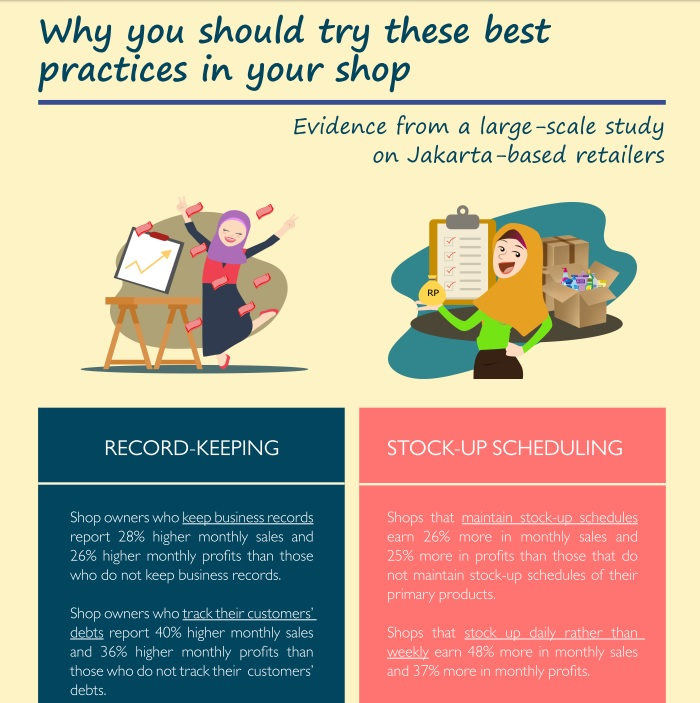
\includegraphics[width=2.6in]{pics/Handbook_return.jpg}
	
	\label{height}
\end{figure}
\end{frame}


\begin{frame}
\frametitle{Handbook Content}

\begin{figure}[htbp]
	\centering
		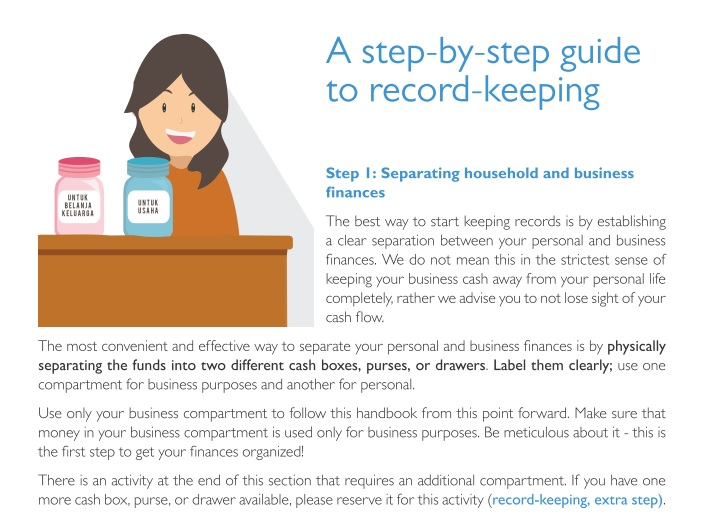
\includegraphics[width=2.6in]{pics/Handbook_stepbystep.jpg}
	
	\label{height}
\end{figure}
\end{frame}

\begin{frame}
\frametitle{Movie with Successful Peers}
\begin{figure}[htbp]
	\centering
		\includegraphics[width=4.4in]{pics/movie.jpg}
   
	\label{height}
\end{figure}
\end{frame}


\begin{frame}
\frametitle{Implementation Assistance for Business Practices}
\begin{figure}[htbp]
	\centering
		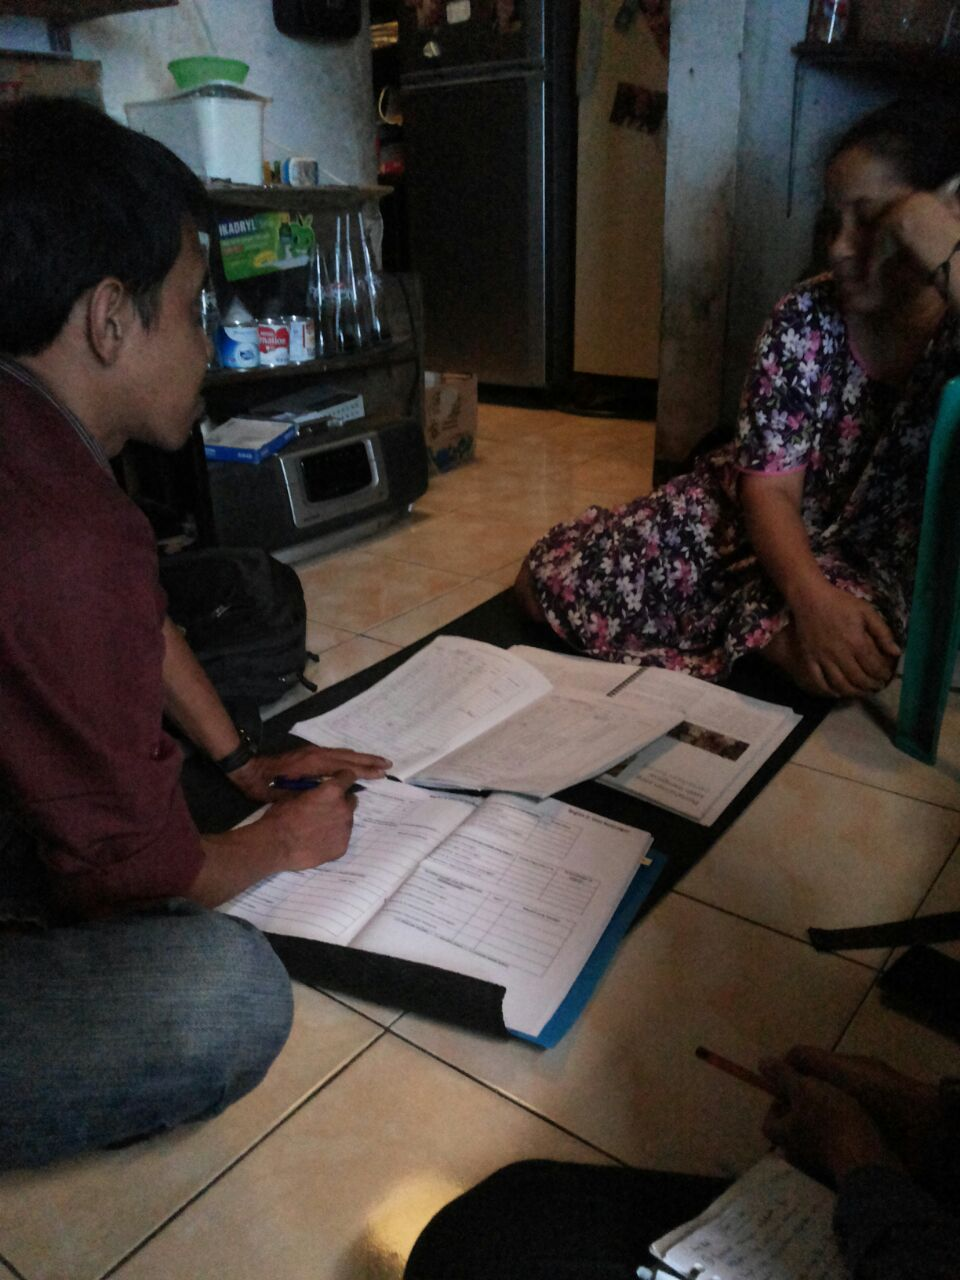
\includegraphics[width=2.0in]{pics/Assistance_expl.jpg}
	
	\label{height}
\end{figure}
\end{frame}


\subsection{Results}

\begin{frame}
\frametitle{Summary Statistics}

%\makebox[\linewidth][c]{
%\begin{tabular}{l cc ddd}


{\tiny{
	\begin{table}
		%\begin{adjustbox}{width=9.6cm}
		\centering	
		\tabcolsep=0.2cm

			\begin{tabular}{l*{10}{c}}
			\hline\hline
			\hline


&\multicolumn{1}{c}{\textcolor{bdf}{Control}}
&&\multicolumn{1}{c}{\textcolor{bdf}{HB only}}	
&&\multicolumn{1}{c}{\textcolor{bdf}{HB \& MOV}	}
&&\multicolumn{1}{c}{\textcolor{bdf}{HB \& HELP}}	
&&\multicolumn{1}{c}{\textcolor{bdf}{HB \& MOV}}	\\


&\multicolumn{1}{c}{}
&&\multicolumn{1}{c}{}	
&&\multicolumn{1}{c}{}
&&\multicolumn{1}{c}{}	
&&\multicolumn{1}{c}{\textcolor{bdf}{\& HELP}}	\\


&\textit{N = 261}	
&&\textit{N = 260}	
&&\textit{N = 260}	
&&\textit{N = 260}	
&&\textit{N = 260}	\\
\hline \\

\textcolor{bdf}{Firm Owner Characteristics} \\
Gender (Male=1)											& 0.28	&& 0.3	&&0.29	&& 0.3	&& 0.28\\
Age														&45.22	&&45.27	&&45.28	&&45.16	&&45.38 \\
Education (Years)										&9.1	&&9.52	&&9.36	&&9.42	&&9.55 \\
%Digitspan												& 1.7	&& 1.67 && 	1.8 &&	1.67	&& 1.69 \\
														%&(1.12) 	&& 		&& 		&& 		&& 		&& \\
Risk Preference (0 - 10 ``Perfectly Risk-Seeking'')		&3.74	&&3.76	&&3.88	&&3.6	&&3.68 \\											
Time Preference	(0 - 10 ``Perfect Patience'')			&5.19	&&5.07	&&5.21	&&5.25	&&5.2 \\[0.5ex]
\\														
\textcolor{bdf}{Firm Characteristics} \\
Firm Age (Years)										&12.76		&&13.77		&&14.03		&&13.98		&&13.47 \\
Family Member Is Business Partner							&0.56		&&0.6		&&0.63		&&0.59		&&0.62 \\
Total Number of Workers									&2.03		&&2.05		&&1.9		&&1.99		&&2.04 \\
%Number of Full Time Paid Employees						&0.09		&&0.1		&&0.08		&&0.08		&&0.11		&&0.08 \\
														%&(0.3)		&&			&&			&&			&&			&& \\
Business Has Tax ID										&0.2		&&0.21		&&0.2		&&0.15		&&0.18 \\
Total Sales Last Month (USD PPP)						&4454.37 &&	4730.64	&& 4840.55	&& 4761.4	&& 5139 \\
												
Total Profits Last Month (USD PPP)						& 889.58	&& 961.1 &&	926.78	&& 825.25	&& 934.66 \\
Applied for Bus Loan in Last 12 Months
			    & 0.2	&& 0.17	&& 0.15	&& 0.22	&& 0.17 \\
													
Obtained Bus Loan in Last 12 Months
						& 0.18 &&	0.15	&& 0.14	&& 0.18	&& 0.14 \\[0.5ex]
\\
\\
\textcolor{bdf}{Business Practices} \\
Management Practices Aggregate Score											& 0.37	&& 0.36	&& 0.37	&& 0.35	&& 0.37 \\
\hspace{3mm}Marketing Subscore												& 0.23	&& 0.23 &&	0.25	&& 0.23	&& 0.24 \\
\hspace{3mm}Stocking-up	Subscore											& 0.45	&& 0.47	&& 0.47	&& 0.47	&& 0.46 \\
\hspace{3mm}Record-keeping Subscore											& 0.33	&& 0.28	&& 0.3	&& 0.29 &&	0.3 \\
\hspace{3mm}Financial-planning Subscore									& 0.51	&& 0.47	&& 0.47	&& 0.43	&& 0.47 \\
%\hspace{3mm} Discussion Subscore                        & 0.57	&& 0.59	  && 0.61	&& 0.6	&& 0.64  \\
&		&&		&&		&& \\
		\hline
		\hline
			\end{tabular}
		%\end{adjustbox}			
		
		%\begin{adjustbox}{center}
			%\begin{tabular}{l*{12}{l}}
			%\multicolumn{13}{p{0.95\textwidth}}{\footnotesize \textit{Notes}: $^1$ Last month's sales and profits appear with both tails winsorized at 1%.}
			%\end{tabular}
		%\end{adjustbox}	
		
	\end{table}}}
%\end{tabular}
%\begin{itemize_2pt}
%\item Test of Joint Orthoganality from Multinomial Logit (P-value): 0.857
%\end{itemize_2pt}
\end{frame}


\begin{frame}
\frametitle{Movie: Take Up and Assessment}
{\scriptsize{\begin{table}[htbp]
%\fontsize{10}{11}\selectfont
  \centering
 %   \tabcolsep=0.10cm
    %\begin{adjustbox}{width=11cm}
    \begin{tabular}{lcc}
    \hline
   	& (1)   					&(2)   						 \\
    \hline
  	& \textcolor{bdf}{HB \& MOV} 		& \textcolor{bdf}{HB \& MOV}		  \\
  	& 							& \textcolor{bdf}{\& HELP}			\\
   	& \textcolor{bdf}{(A)}   			& \textcolor{bdf}{(B)}   			 \\
 	&							&							\\
% 	&							&							&& \textit{F-test}\\
   	%	& Assigned 				& Assigned 					&&  \\
   	& \textit{N=260} 			& \textit{N=260} 			 \\
   \hline
   														&		&		 \\
    \textcolor{bdf}{Attendance} 								&       &         \\
  	% 													&		&		&& \\
    Business Owner or Partner Attended Film Screening 	& 0.52  & 0.49   \\
    %Baseline respondent attended film screening 		& 0.47  & 0.45  && 0.792 \\
   	%Respondent was reminded by phone 					& 0.05  & 0.07  && 0.355 \\
    %Respondent was reminded by visit to business 		& 0.35  & 0.33  && 0.782 \\
    %Distance to screening location (in decimal degrees)& 0.01  & 0.01  && 0.869 \\
	&       &       \\
    \textcolor{bdf}{Evaluation (1-4 Scale):}	&       &        \\
   	%									&       &       &&  \\
    Has Learned Something New	& 3.34  & 3.21  \\
    Feels Inspired 				& 3.31  & 3.30   \\
    Feels Hopeful 				& 3.60  & 3.42   \\
    Feels Bored 				& 0.83  & 0.97    \\
    \end{tabular}
   % \end{adjustbox}

\end{table}}}

\end{frame}


%%% Attendance and feedback to assistance + comparison between experimental groups
\begin{frame}

\frametitle{Assistance: Take Up and Assessment}
{\scriptsize{\begin{table}[htbp]
%\fontsize{10}{11}\selectfont
  \centering
    %\tabcolsep=0.10cm
   % \begin{adjustbox}{width=11cm}
    \begin{tabular}{lcc}
    \hline
    & (1)   			& (2) 			\\
    \hline
   	& \textcolor{bdf}{HB \& HELP} 		& \textcolor{bdf}{HB \& MOV,}		 \\
  	& 							& \textcolor{bdf}{\& HELP}			 \\
   	& \textcolor{bdf}{(A)}   			& \textcolor{bdf}{(B)}   			\\
	&							&							 \\
% 	&							&							&& \textit{F-test}\\
   	%	&& Assigned 				& Assigned 					&&  \\
   	& \textit{N=260} 			& \textit{N=260} 		\\
    \hline
          																				&       &      \\
    \multicolumn{1}{l}{\textcolor{bdf}{Attendance}} 											&       &        \\
    %\multicolumn{1}{l}{\textit{1st session}} 											&       &       & &  \\
    \multicolumn{1}{l}{    Business Owner or Partner Attended 1st Session} 				& 0.77  & 0.78  \\
    %\multicolumn{1}{l}{    Baseline respondent attended 1st session} 					& 0.76  & 0.77  && 0.756 \\
    %\multicolumn{1}{l}{    Recipient plans to use at least one new practice} 			& 0.37  & 0.47  && 0.021** \\
    %\multicolumn{1}{l}{    Recipient plans neither handbook study nor implementation} 	& 0.12  & 0.11  && 0.784 \\
         														 						%&     	&       &&  \\
    %\multicolumn{1}{l}{\textit{2nd session}} 											&       &       &&  \\
    \multicolumn{1}{l}{    Business Owner or Partner Attended 2nd Session} 				& 0.68  & 0.68   \\
    %\multicolumn{1}{l}{    Baseline respondent attended 2nd session} 					& 0.67  & 0.67  && 1 \\
    %\multicolumn{1}{l}{    Recipient plans to use at least one new practice} 			& 0.39  & 0.47  && 0.063* \\
    %\multicolumn{1}{l}{    Recipient plans neither handbook study nor implementation} 	& 0.13  & 0.08  && 0.044** \\
          																				&       &        \\
    \multicolumn{1}{l}{\textcolor{bdf}{Evaluation (1-4 Scale)}} 								&       &         \\
    \multicolumn{1}{l}{Has Learned Something New} 										& 2.88  & 2.89   \\
    \multicolumn{1}{l}{Feels Inspired} 													& 2.76  & 2.83   \\
    \multicolumn{1}{l}{Feels Hopeful} 													& 2.88  & 2.97  \\
    \multicolumn{1}{l}{Feels Bored} 													& 0.59  & 0.43   \\
    \end{tabular}
   % \end{adjustbox}

\end{table}}}
\end{frame}


\begin{frame}
\frametitle{Impact on Business Practices}
\framesubtitle{Aggregate Scores}
{\tiny{\begin{table}[t]
%\centering
%\begin{adjustbox}{width=10cm}
%	\tabcolsep=0.05cm
	\begin{tabular}{l*{10}{c}}
		\hline \hline
		\\
			&\textcolor{bdf}{Record}			&&\textcolor{bdf}{Planning}			&&\textcolor{bdf}{Stocking-up}	&&\textcolor{bdf}{Marketing} && \textcolor{bdf}{Joint} \\
&\textcolor{bdf}{Keeping}                       &&                        &&	                   &&	 && Decision-making \\
					&(1)					&&(2)						&&(3) 						&&(4) && (5)\\
			\cline{2-2}					\cline{4-4}					\cline{6-6}			\cline{8-8} \cline{10-10}  \\


Assigned Handbook 			&                    0.025   &&	          0.027   	 &&           -0.007   	 &&          -0.011   	  &&         0.011
      \\
         							&               (0.209)   	   &&      (0.273)   	&&         (0.694)   	     &&    (0.694)   	&&         (0.694)
    \\

         							
Assigned Handbook \& Movie 	&                     0.057*** 	 &&          0.043  	   &&       0.038  	    &&       0.040    &&        0.040        \\
          							&              (0.009)   &&	         (0.107)   	  &&       (0.117)   	  &&       (0.166)   	 &&        (0.217)         \\

         							
Assigned Handbook \& Assistance 	&              0.065*** 	  &&         0.034   	&&           0.011   	 &&           0.039 	       &&      0.037    \\
         							&           (0.004)   	  &&       (0.166)   &&	         (0.664)   && 	         (0.166)   	  &&       (0.239)    \\

         							
Assigned All Three          	&                0.054***	  &&         0.068***  	 &&          0.053**  	    &&       0.061**	   &&        0.059*          \\
									&             (0.009)    &&	         (0.009)   	&&         (0.020)   	  &&       (0.032)   &&	         (0.094)           \\

\hline         							
\\
R-squared									&               0.204   	 &&          0.192   	&&           0.187   	&&           0.150	 &&           0.120             \\
Sample Size 								&               2205   	  &&          2204   	   &&         2205   	 &&           2205   	    &&        2205      \\
Dependent Variable Mean of Control 		&                  0.196  	  &&         0.402   	 &&          0.471    &&	           0.250    	 &&          0.269          \\
Dependent Variable SD of Control 			&              0.252    	 &&          0.310   	  &&         0.270      	  &&         0.320    && 	           0.420        	\\
F-tests (p-value):							&			&&			&&			&&			\\
\hspace{5mm}Book = Book \& Mov				        &               0.069   	   &&           0.487   	  &&          0.014     	  &&          0.028    	 &&          0.300           \\
\hspace{5mm}Book = Book \& Assistance				        &               0.025  	  &&          0.754     	 &&           0.304   	 &&          0.030    	  &&          0.348                 \\
\hspace{5mm}Book = All Three				        &                  0.096    	  &&         0.073    	    &&      0.001   	  &&         0.002    &&	         0.082        \\
\hline
	\end{tabular}
%\end{adjustbox}
\end{table}}}
\begin{itemize_2pt}
\item Multiple hypothesis testing corrected p-values in parentheses
\item "All Three" improvement of 28 \% in record-keeping, 17 \% in planning, 11 \% in stocking, 24 \% in marketing and 22 \% in joint decision making.
\end{itemize_2pt}
\end{frame}


\begin{frame}

\frametitle{\centering{Business Profits}}
{\scriptsize{\begin{table}[t]
\centering
%\begin{adjustbox}{width=9cm}
%	\tabcolsep=0.05cm
	\begin{tabular}{l*{5}{c}}
\hline
\hline
			   &&Profits	        &&Profits \\
				&&last month  		&&last month \\
			&&(win 5\%)			&&(IHS) \\
				&&(1)				&&(2)	\\
&& \\
					\hline
&&\\
		

Assigned Handbook 					&&-91.307   	&& -0.067   		\\
       								 	&&         (78.400)  	&&          (0.088)  	\\

         							
Assigned Handbook \& Movie				&&110.378   	  	&& 0.055   		\\
       									&&         (86.841)  	&&          (0.092)  	\\

         							
Assigned Handbook \& Assistance 	&&         310.455***	&&           0.261***		\\
       								 	&&         (89.488) 	&&          (0.096)  	\\
         							
Assigned All Three          		&&         191.088**  	&&           0.199** 		\\
       								 	&&         (84.662)  	&&          (0.094)  	\\

   	\\
\hline         							
\\
R-squared											  	&& 0.179  	&& 0.211  	\\
Sample Size 											&&2172	&& 2172 	\\
Dependent Variable Mean in Control Group			 	&&          894.544   	&&           6.817 	\\
Dependent Variable SD in Control Group				 	&&         1127.783   	 &&          1.348  	\\
F-tests (p-value):											&&			&&			\\
\hspace{5mm}Book = Book \& Mov				        	&&    0.020   	&&            0.167 	\\
\hspace{5mm}Book = Book \& Assistance				  			&&0.000   	&&0.000  	\\
\hspace{5mm}Book = All Three			   			  	&&0.001   	&&0.003  	\\
\hline
	\end{tabular}
%\end{adjustbox}

\end{table}}}
\begin{itemize_2pt}
\item Profits increase by 35\% (about 0.28 sd.) - ITT.
\end{itemize_2pt}
\end{frame}




\begin{frame}
\frametitle{Business Sales}
{\scriptsize{\begin{table}[t]
\centering
%\begin{adjustbox}{width=9cm}
%	\tabcolsep=0.05cm
	\begin{tabular}{l*{5}{c}}
\hline
\hline
                &&ITT	        &&TOT \\
			   &&Sales	        &&Sales \\
				&&last month  		&&last month \\
			&&(win 5\%)			&&(win 5\% \\
				&&(1)				&&(2)	\\
&& \\
					\hline
&&\\
		

Assigned Handbook 					&&-396.976   	&&               -417.198		\\
       								 	&&        (314.252)   	&&          -417.198	\\

         							
Assigned Handbook \& Movie				&&335.489   	  	&& 601.221    		\\
       									&&       (337.881)  	&&            (606.634)	\\

         							
Assigned Handbook \& Assistance 	&&                   836.755**	&&                     1031.692** 	\\
       								 	&&        (372.924) 	&&            (457.015) 	\\
         							
Assigned All Three         		&&         807.462**  	&&                         1558.326**		\\
       								 	&&        (358.384)  	&&          (696.317)   	\\

   	\\
\hline         							
\\
R-squared											  	&& 0.492  	&&  0.483	\\
Sample Size 											&& 2197	&& 2197 	\\
Dependent Variable Mean in Control Group			 	&&         4998.923   &&	          4998.923 	\\
Dependent Variable SD in Control Group				 	&&         5623.257   	&&           5623.257	\\
F-tests (p-value):											&&			&&			\\
\hspace{5mm}Book = Book \& Mov				        	&&            0.020 	&&           0.047 	\\
\hspace{5mm}Book = Book \& Assistance				  			&&0.000   	&& 0.000 	\\
\hspace{5mm}Book = All Three			   			  	&&0.000   	&&0.001  	\\
\hline
	\end{tabular}
%\end{adjustbox}

\end{table}}}
\begin{itemize_2pt}
\item Sales increase by 16\% (about 0.15 sd.) - ITT %- and 31\% (0.28 sd.) - TOT.
\end{itemize_2pt}
\end{frame}


\begin{frame}
\frametitle{Other Outcomes}
\begin{itemize_2pt}
\item \textcolor{bdf}{No significant} impacts on:
    \begin{itemize_2pt}
    \vspace{0.1in}
    \item Business expenses
    \vspace{0.1in} 		
    \item Size of the shop
      \vspace{0.1in}
    \item Number of employees
      \vspace{0.1in}
    \item Number of customers
       \vspace{0.1in}
     \item Business credit
    \end{itemize_2pt}
\end{itemize_2pt}
\end{frame}

\subsection{Discussion}
\begin{frame}
\frametitle{Efficiency Gains?}
Impact on business practices $\rightarrow$ \textcolor{bdf}{efficiency practices}:
\vspace{0.1in}
\begin{itemize_2pt}
	\item Adjust stocks based on product profitability
	\item Negotiate lower prices with suppliers
	\item Consult with former customers
	\item Offer discounts
	\item Make joint decisions
	\item Review performance to identify ways to improve
	\item Make anticipated budget for upcoming costs

	\pause
	
	\item[] $\rightarrow$ \textcolor{bdf}{Non-record-keeping practices}
	\item[] $\rightarrow$ \textcolor{bdf}{Stocking up and marketing practices} appear to drive performance effects (causal-mediation analysis)
	\item[] $\rightarrow$ Variance in profits among treated firms does not converge
	\item[] $\rightarrow$ \textcolor{bdf}{Efficiency gains}
\end{itemize_2pt}
\end{frame}

\begin{frame}
\frametitle{Business Knowledge or Aspirations?}
Impact on practice adoption and business performance may work through ..
\begin{itemize_2pt}
	\item .. acquisition of \textcolor{bdf}{business knowledge} and/or
	\item .. strengthening of \textcolor{bdf}{business aspirations}
\end{itemize_2pt}

\pause
\vspace{1.0em}

We directly measure \textcolor{bdf}{business aspirations} .. 
\begin{itemize_2pt}
	\item .. at baseline, midline, and endline
	\item .. for short (one year) and long ("ideal business") time horizons
	\item .. for various dimensions of potential business expansion
    \begin{itemize_2pt}
   		\item Sales on a normal day
    	\item Physical size
   		\item Customers on a normal day
    	\item Employees
    \end{itemize_2pt}
\item[] $\rightarrow$ \textcolor{bdf}{No impact on aspirations}
\item[] $\rightarrow$ Performance likely driven by increase in \textcolor{bdf}{business knowledge}
\end{itemize_2pt}

\end{frame}

\begin{frame}
\frametitle{Business Stealing?}
Do treated businesses improve performance at the expense of the control?
\vspace{0.1in}
\begin{itemize_2pt}
\item Sales and profits of \textcolor{bdf}{control businesses do not decrease} from baseline to endline (roughly equal)
\item Sales and profits of control businesses \textcolor{bdf}{closer to treated shops do not decrease by more} than those further away
\item[] $\rightarrow$ \textcolor{bdf}{No evidence for business stealing}
\end{itemize_2pt}
\end{frame}

\begin{frame}
\frametitle{Cost-Effectiveness}

\textcolor{bdf}{Small costs (per firm)}:
\begin{itemize_2pt}
\item Cost Handbook alone: USD 100
\item Cost Handbook \& Movie: USD 125
\item Cost Handbook \& Assistance: USD 125
\item Cost Handbook \& Movie \& Assistance: USD 150
\end{itemize_2pt}
\vspace{0.5em}

\textcolor{bdf}{Substantial Benefits}
\begin{itemize_2pt}
\item Up to USD 330 per month in profits
\item Adoption of top practices by retailers
\end{itemize_2pt}

\vspace{0.5em}
Research design likely \textcolor{bdf}{scalable and portable}

\end{frame}

\subsection{Conclusion}
\begin{frame}
\frametitle{Takeaways}
\begin{itemize_2pt}
    \item \textcolor{bdf}{Curating local knowledge has value for business growth} 
    \item Information alone does not have impact, only combined with \textcolor{bdf}{behavioral interventions}
    \item Mechanism likely \textcolor{bdf}{knowledge-based}, not aspirations-based
	\item Behavioral interventions are \textcolor{bdf}{inexpensive and scalable}
	\item[] $\rightarrow$  Attractive for policy
    
\end{itemize_2pt}
\end{frame}





%\addtocontents{toc}{\protect\setcounter{tocdepth}{0}}

\appendix
\begin{frame}[label=references, allowframebreaks]
\frametitle{References}
\bibliographystyle{econometrica}
\bibliography{SME_library}
\end{frame}


\section*{\textbf{APPENDIX}}

\setbeamertemplate{sidebar right}[sidebar theme]

%\begin{frame}{Appendix Overview}
%\tableofcontents[currentsection,hideothersubsections]
%\end{frame}


\begin{frame}[label=McK2020_sales]
\frametitle{Evidence of Impact}

	\begin{figure}[htbp]
		\centering
		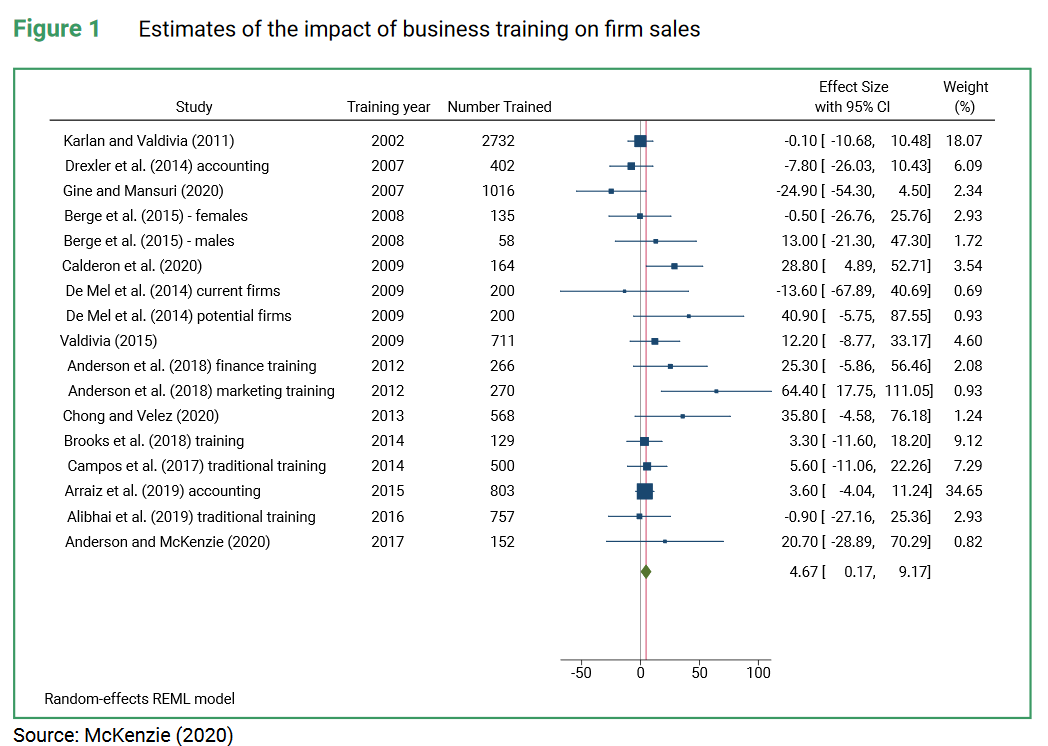
\includegraphics[width=23.2em]{pics/McK2020_sales.png}
		\label{McKenzie(2020): Sales}
	\end{figure}	
	
	\vspace{-1em}	
	
	\begin{itemize_2pt}
		\item Small positive impact on sales (back to \hyperlink{McK2020_profits}{\beamergotobutton{profits}})
	\end{itemize_2pt}
	
\end{frame}


\end{document}
